\chapter{Introduction}

\section{Proteins and Protein Folding}

\subsection{Protein Structure Prediction - Motivation}
    
Proteins are one of the essential cellular macromolecules, together with DNA, RNA, saccharides, lipids and others.
They perform a variety of functions inside and outside of cells as receptors, enzymes, antibodies, hormones, structural components, transporters, etc. 

At the ground level proteins are composed of chained amino acids, which are connected through peptide bonds. 
There are more than thousand of known amino acids occurring in nature, however, only 22 of them are involved in protein assembly - proteinogenic (21 in eukaryotes). 
Twenty of these amino acids are encoded by DNA; their name and one-letter code are shown in Table \ref{tab:aa_codes} \cite{protgenaa}. 
The sequence of amino acids is called the primary structure of a protein.

\begin{table}
    \centering
    \begin{tabular}{r|c|r|c|}
        Alanine & A & Arginine & R \\
        Asparagine & N & Aspartic acid & D \\
        Cysteine & C & Glutamine & Q \\
        Glutamic acid & E & Glycine & G \\
        Histidine & H & Isoleucine & I \\
        Leucine & L & Lysine & K \\
        Methionine & M & Phenylalanine & F \\
        Proline & P & Serine & S \\
        Threonine & T & Tryptophan & W \\
        Tyrosine & Y & Valine & V
    \end{tabular}
    \caption{Standard amino acid abbreviations}
    \label{tab:aa_codes}
\end{table}

To perform their function proteins fold into stable three-dimensional structures in a very dense and fast-changing environment.
This three-dimensional structure is also called the tertiary structure of the protein. 
On the lower level, the secondary structure describes local folds of amino acids, where the 3 basic classes are Helices, Sheets and Coils.
The very delicate conformation of the protein is crucial for the correct functioning of the cell.
In rare cases, when the structure is corrupted, it might result in serious diseases such as cystic fibrosis, Parkinson's disease, Huntington's disease, cancer and many others \cite{protein_misfolding_diseases}.

It is hypothesized that the instructions for the folding are encoded in the primary protein structure. 
The thermodynamic theory states, that if a denatured protein occurs in an environment it was selected for (pH, ionic strength, etc.) then it will fold into a state with minimum Gibbs free energy.
This state is also called a "native state" of a protein. 
Christian B. Anfinsen and his group published a famous paper in 1973, where they managed to denature ("unfold") a protein (bovine pancreatic ribonuclease) with urea - shown in Figure \ref{fig:primarytertiary}a). 
Afterwards, when they removed urea the protein folded back into the same state as the initial one \cite{anfinsen}. 
This suggests a link between the primary and tertiary structure which has to be uncovered. 
Although the progress in the past few decades, the prediction of novel amino acid sequences remains a great challenge, mainly due to the high complexity of the problem.

\begin{figure}[b!]
    \centering
    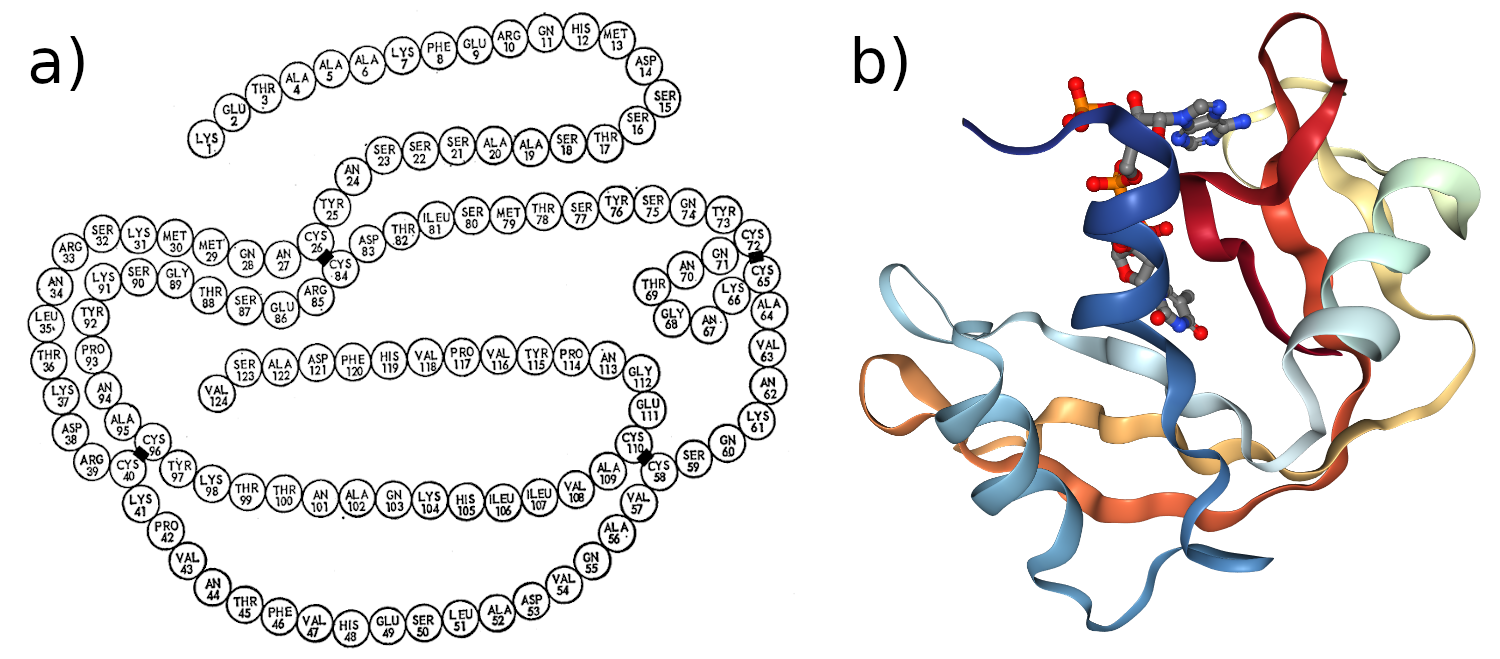
\includegraphics[width=\linewidth]{imgs_tomas/primary_tertiary.png}
    \caption{Primary (a)) \cite{anfinsen} and tertiary structure (b)) \cite{pdb} of bovine pancreatic ribonuclease.}
    \label{fig:primarytertiary}
\end{figure}

Experimental approaches to obtaining the spatial structure include X-ray crystallography and Nuclear Magnetic Resonance (NMR) with the former being responsible for the majority of known structures. 
Since the relative distances between amino acids are in order of \AA ngstroms ($\sim10^{-10}$m), visible light ($\sim10^{-7}$m) can not be used to observe the structures, hence the higher energy X-rays which operate within this region. 
Major disadvantages of experimental techniques are their high cost ($\sim 10,000\mathdollar-1,000,000\mathdollar$) and low success rate ($\sim 10\%-50\%$) \cite{protcost}.
The ability to determine the tertiary structure of a protein with better accuracy would help especially in medicine and research, by designing new ones to battle with diseases as drug vectors.
These are good reasons for trying to develop computational methods for determining protein structure and avoid these time and money consuming steps.
However, due to the vast structure search space, it is impossible to develop an exact optimization algorithm working on current computers.

To get an idea of how difficult the problem of structure prediction is, let us consider a simple scenario. 
Assume that we have protein of length 100 and each amino acid residue consists of two rotatable bonds. 
For simplicity, we will focus on the problem of minimizing an Energy function (Gibbs free energy).
If there were only 2 allowed angles per rotatable bond, then the total number of possible conformations is $(2\cdot2)^{100} = 4^{100}$. 
If we had a computer that can generate one of these unique conformations, compute its Gibbs energy and check whether it is smaller than the current minimum in a picosecond ($10-{12} s$), than to find the optimal structure would take roughly $5 \cdot 10^{43}$ years (the universe is $\sim 13.8\cdot10^9$ years old).

\subsection{Amino acids}

\begin{figure}
    \centering
    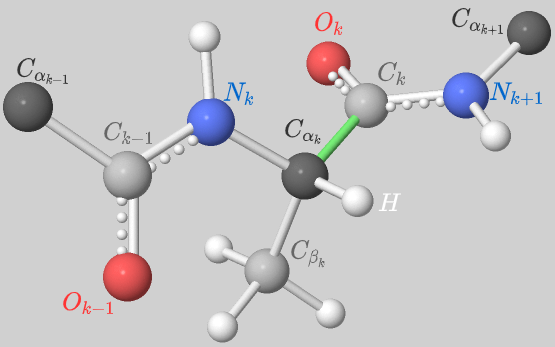
\includegraphics[scale=0.5]{imgs_tomas/backbone.png}
    \caption{Protein backbone with atom names. Modified picture from \cite{ramachandran}}
    \label{fig:backbone0}
\end{figure}

\begin{figure}
    \centering
    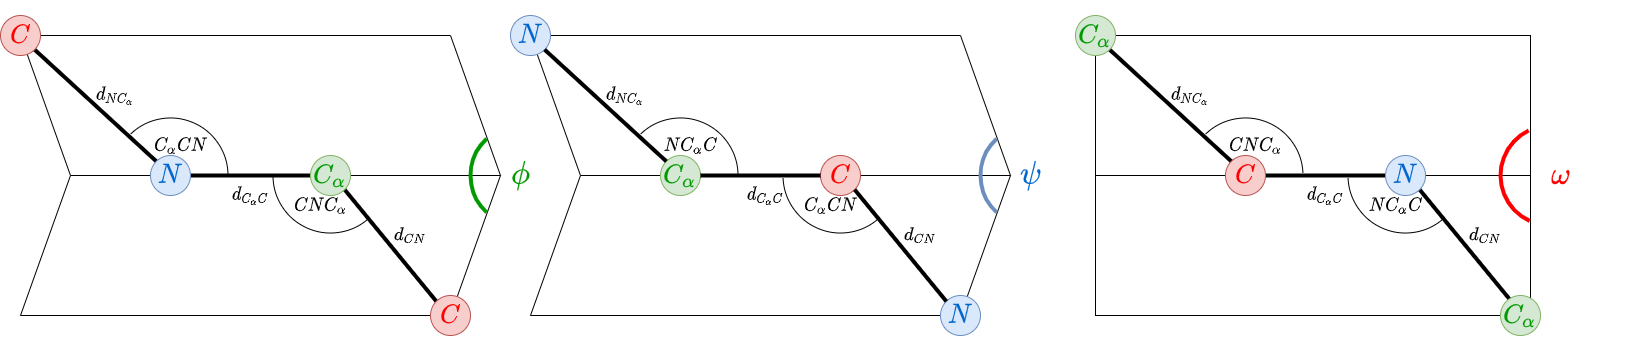
\includegraphics[width=\linewidth]{imgs_tomas/torsion.png}
    \caption{Torsion Angles - planes and inter-atom distance and angles notation}
    \label{fig:torsion}
\end{figure}

Amino acids are organic compounds that are the basic building blocks of proteins. 
22 amino acids are involved in protein generation, 20 of them which are encoded by DNA are also subject to translation processes. 
Structurally, amino acids are composed of two parts (see Figure \ref{fig:backbone0}):

\begin{enumerate}
    \item Backbone
    
        which consists of three atoms: Nitrogen atom - N, alpha Carbon - C$_\alpha$ and a Carbon atom - C
    \item Residue
        
        The amino acid residue is attached to the backbone through a C$_\beta$ - C$_\alpha$ bond. The residue is a unique molecule that distinguishes amino acids from each other. The only amino acid without a residue is glycine, which instead of the C$_\beta$ has a hydrogen atom.
\end{enumerate}

In theory, the bonds between backbone atoms (N - C$_\alpha$, C$_\alpha$ - C and C - N) should be of constant length, as well as the angle defined by a unique set of three consecutive atoms (N - C$_\alpha$ - C, C$_\alpha$ - C - N and C - N - C$_\alpha$). 
Even if this is not completely true, the spreads of the distributions are relatively low, which allows us to treat them as constants.

This assumption leads to the following consequence: since the distances and angles between consecutive atoms are constant, instead of describing the backbone as a list of coordinates, one can use the so-called torsion angles.

Torsion angle, or a dihedral angle, is an angle defined by two intersecting planes. 
Since there are three atoms in the backbone, we can define three pairs of intersecting planes and thus define the three torsion angles (Figure \ref{fig:torsion}). 
Knowing the position of three preceding atoms, the torsion angle $\phi$ defines the position of the next C atom, the torsion angle $\psi$ defines the position of the next N atom and finally $\omega$ defines the position of the next C$_\alpha$ atom. 
The bond between atom C and N in the protein backbone is a peptide bond that behaves similarly to a double bond and is almost always equal to 180\degree~(trans isomerism; 0\degree~for cis configuration). 
This means that for the construction of protein geometry one only requires two torsion angles: $\phi$ and $\psi$.

Figure \ref{fig:ramachandran} a) shows the distribution of these two angles. 
Most of the combinations of the two angles are not allowed due to steric clashes. 

Since the secondary structure of a protein is defined as a "repetitive conformation of the residues and, ultimately, repetitive values of $\phi$ and $\psi$", the two basic secondary structure classes can be distinguished in the Ramachandran plot, with $\alpha$ helix having the distribution in lower left quadrant and $\beta$ sheets in the upper left quadrant (see Figure \ref{fig:ramachandran}). 
Several other classes have been described and their location in the Ramachandran plot can be also localized. These will be described in more detail in the next section. 

\begin{figure}
    \centering
    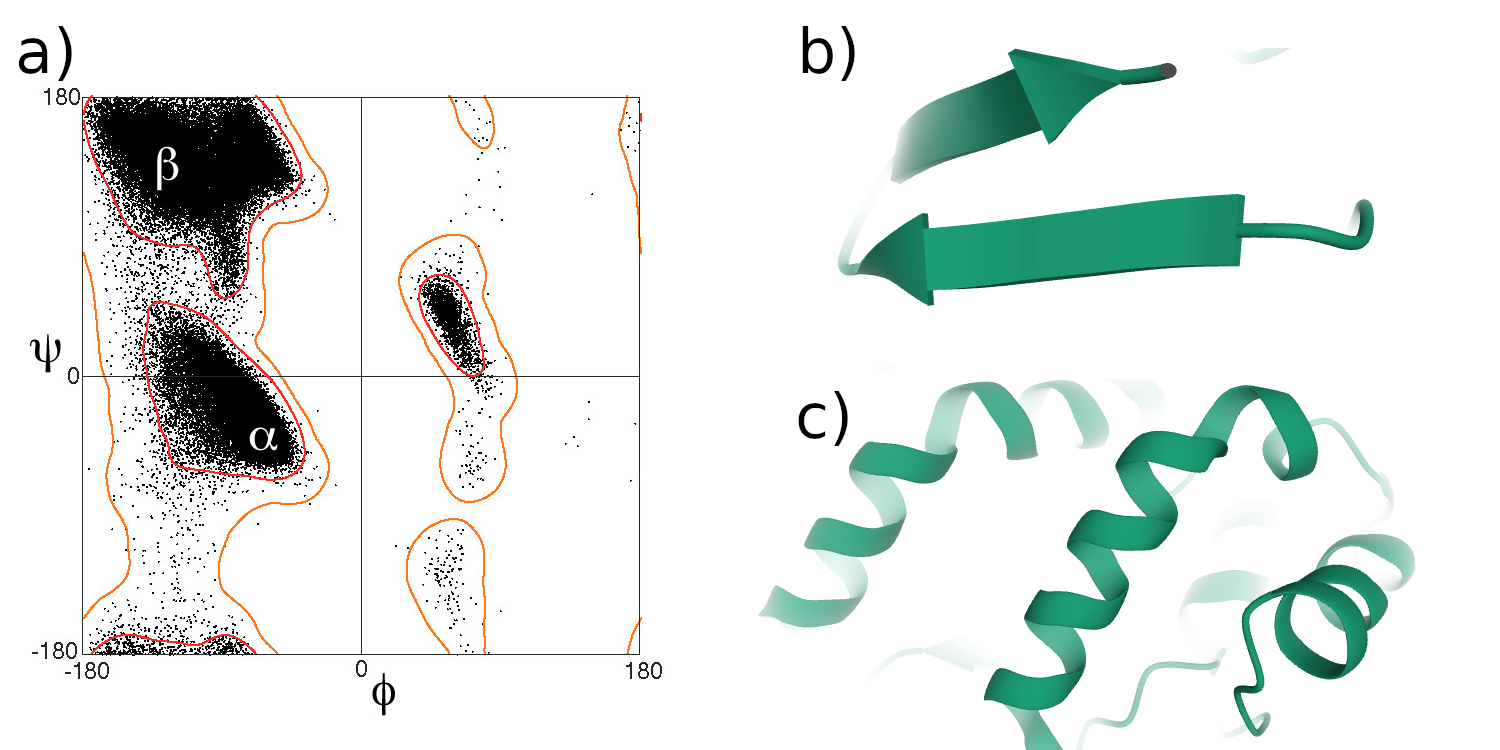
\includegraphics[width=\linewidth]{imgs_tomas/secondary.png}
    \caption{Ramachandran plot \cite{ramachandran} a) and two basic secondary structures - b) a beta sheet and c) an alpha helix \cite{pdb}}
    \label{fig:ramachandran}
\end{figure}

\subsection{Protein Folding}

Protein folding refers to a process of post-translational arrangement of amino acids in the cytoplasm. 
The purpose of this process is to create a favourable structure for performing a specific task, which is dependent on the type of amino acid residues attached to the backbone. 
Proteins are created in cells all the time and the same sequence of amino acids should always result in the same folding process. 
As illustrated in the introduction, the experimental inference of protein structure is both time and money consuming and due to the complexity of the problem, the computational method can only create estimates of the structure.

At the lowest level protein are composed of a sequence of amino acids. 
These sequences then create three-dimensional folds, from which one can derive local repetitive regions - secondary structure. 

Proteins (or protein chains) can also be divided into smaller independently folding regions called domains. 
Domains are responsible for some functionality or interaction with other molecules \cite{domains}.

The main driving forces of protein folding are hydrophobic interactions. 
Every amino acid can be classified either as hydrophilic/polar ("water liking") or hydrophobic. 
The hydrophobic amino acids tend to orient themselves towards the core of the protein, while the polar amino acids are more likely to be oriented towards the surface.

\subsubsection{Secondary structure}

Parts of the folded structure can be classified into either 3 basic local repetitive regions: $\alpha$ helix (Figure \ref{fig:ramachandran} c)), $\beta$ sheet (Figure \ref{fig:ramachandran} b)) and coil or 8 class classification as suggested by Sander and Kabsch in 1983 - DSSP classification \cite{dssp2}. 
There are also other classification schemes, but DSSP seems to be the one most widely used. 
The 8 classes of the DSSP algorithm are derived from the atom coordinates (Table \ref{tab:dssp0} shows them).

\begin{table}[ht]
    \centering
    \begin{tabular}{c|c}
        DSSP code & Secondary Structure\\ 
        \hline
        H     & $\alpha$-helix \\
        B     & Isolated $\beta$-bridge residue \\
        E     & strand \\
        G     & $3_{10}$ helix \\
        I     & $\Gamma$-helix \\
        T     & Turn \\
        S     & Bend \\
        -     & Other 
    \end{tabular}
    \caption{DSSP Secondary Structure Classes}
    \label{tab:dssp0}
\end{table}

Since the secondary structure elements are stabilized by hydrogen bonds, the algorithm is based on recognition of hydrogen bonding patterns between the C-O bond of one residue and N-H bond of residue three to five residues away \cite{dssp2}. 
A reclassification from 8 state to 3 state secondary structure is possible, where G, H and I are Helices, B and E are sheets and T, S, and - are coils. 
The state of the art performance of 3-state (Q3) secondary structure classifiers is $~84\%$, achieved by models based on neural networks. 
For the 8 class classification, $71\%$ was achieved by an ensemble of 10 models, each of which consisted of a combination of convolutional and recurrent neural network layers \cite{dssp_sec}. 

\subsection{Tertiary structure}

The tertiary structure of a domain/protein is the result of the folding process. 
It is a 3-dimensional conformation of densely packed amino acids with free energy as low as possible. 
As already stated above, this process is driven mainly by hydrophobic interactions. 
Other forces that stabilize the structure are the hydrogen bonds (which give rise to the secondary structure elements), Van der Waals forces or disulfide bridges. 
On top of this, several folding factors aid the process such as chaperones, oxidoreductases, glycan-binding protein and other \cite{principles_of_pf}.

\subsection{Current Approaches to (ab initio) protein folding}

Deep learning has been showing great results and potential in a variety of applications since $\sim2012$, and the protein folding community noticed this (especially during CASP12 - 2016 and CASP13-2018). 
However several very good performing methods were developed applying the laws of physics and molecular dynamics or clever search through libraries of fragmented parts of tertiary structures. 
Due to the large number of unique discovered protein sequences the evolutionary point of view can be applied to the problem by observing conserved pairs of sites. 
In the last few years, the area of quantum computing has been developing and there is a definite potential of using these methods for optimizing protein folds. 
The principle of these 4 methods will be sketched out in the following paragraphs.

\subsubsection{Energy based methods}

As the name suggests, the main goal of these methods is to minimize the free energy of a protein. 
The premise of the method is to use known physical laws and apply them to the folding without requiring knowledge about other structures. 
However, although the promising idea, as shown in the introduction the complexity of the problem is just too large, to allow these methods to arrive at exact solutions.

An example of an energy minimization method is the CSA protocol \cite{csa} (Conformational Space Annealing), which searches the vast conformational energy landscape. 
The algorithm simultaneously optimizes several configurations, compares them against each other and saves the one with minimal energy.

\subsubsection{Fragment Assembly}

The principle of fragment assembly is to use fragments of known structure, stick them together and optimize some energy function. 
Since entire fragments are used, the short-range interactions are not included in the energy function and only long-range are of interest. 
The final result is highly dependent on the choice of the energy function and the optimization procedure \cite{fragments}.

Pipelines of several teams competing at CASP are based on fragment assembly, e.g. I-Tasser developed by Zhang group \cite{zhang} or Rosetta that uses Monte Carlo to assemble the fragments \cite{rosetta}.

\subsubsection{Co-evolutionary features}

Due to the large increase of sequenced primary protein structures, it is possible to look for pairwise amino acids correlations and use them to model the contacts or distances between residues.
Given a set of database primary structures of proteins from different species, we should be able to construct clusters of proteins belonging to the same family (homologs). 
These proteins are likely performing similar functions in different species and should have similar tertiary structures. 
Given a random amino acid sequence we should be able to find similar sequences and construct the Multiple Sequence Alignment - MSA, inside which we should observe linked sites (sites where the correlation of amino acids is far from random). 
Non-random site linkage might be a result of selective pressure (region of the protein responsible for a certain function), direct contact between two non-covalently linked amino acids or indirect/mediated contact between two amino acids. 
Thus it is believed that the MSA holds information about the spatial proximity of amino acid pairs.

The inferred contact or distances are then used as a constraint for the final step in the pipeline - structure optimization. 
AlphaFold developed their structure realization system by optimizing a custom potential function of a protein geometry derived from distance predictions, torsion angle predictions and a score2-smooth potential to prevent steric clashes (foul combinations of torsion angles - see Ramachandran plot: Figure \ref{fig:ramachandran}).

Other best performing teams on CASP (see next section) also adopted this strategy, especially in connection with deep learning, such as Multicom \cite{multicom} or RaptorX \cite{raptorx}

\subsubsection{Quantum Computing}
A recent development in the quantum computing field sparked an interest to apply these new methods to the protein folding problem.
In principle, protein folding on quantum computer uses a very similar formulation of the problem as the energy-based methods.
To search over the vast space of possibilities, the classical computers are forced to perform an exhaustive search, a heuristic search or a deterministic optimization algorithm.
The main difference is that quantum computers allows to represent all the possible solutions as a superposition of quantum states. 
The quantum annealing algorithm can be then used to shift the probability of sampling the globally optimal solution up \cite{mulligan2019designing}.
Currently, the accuracy of this approach is comparable to the energy-based methods, although we expect it to improve significantly in the future as the field of quantum computing will become more mature.  

\subsection{CASP}

\begin{figure}
    \centering
    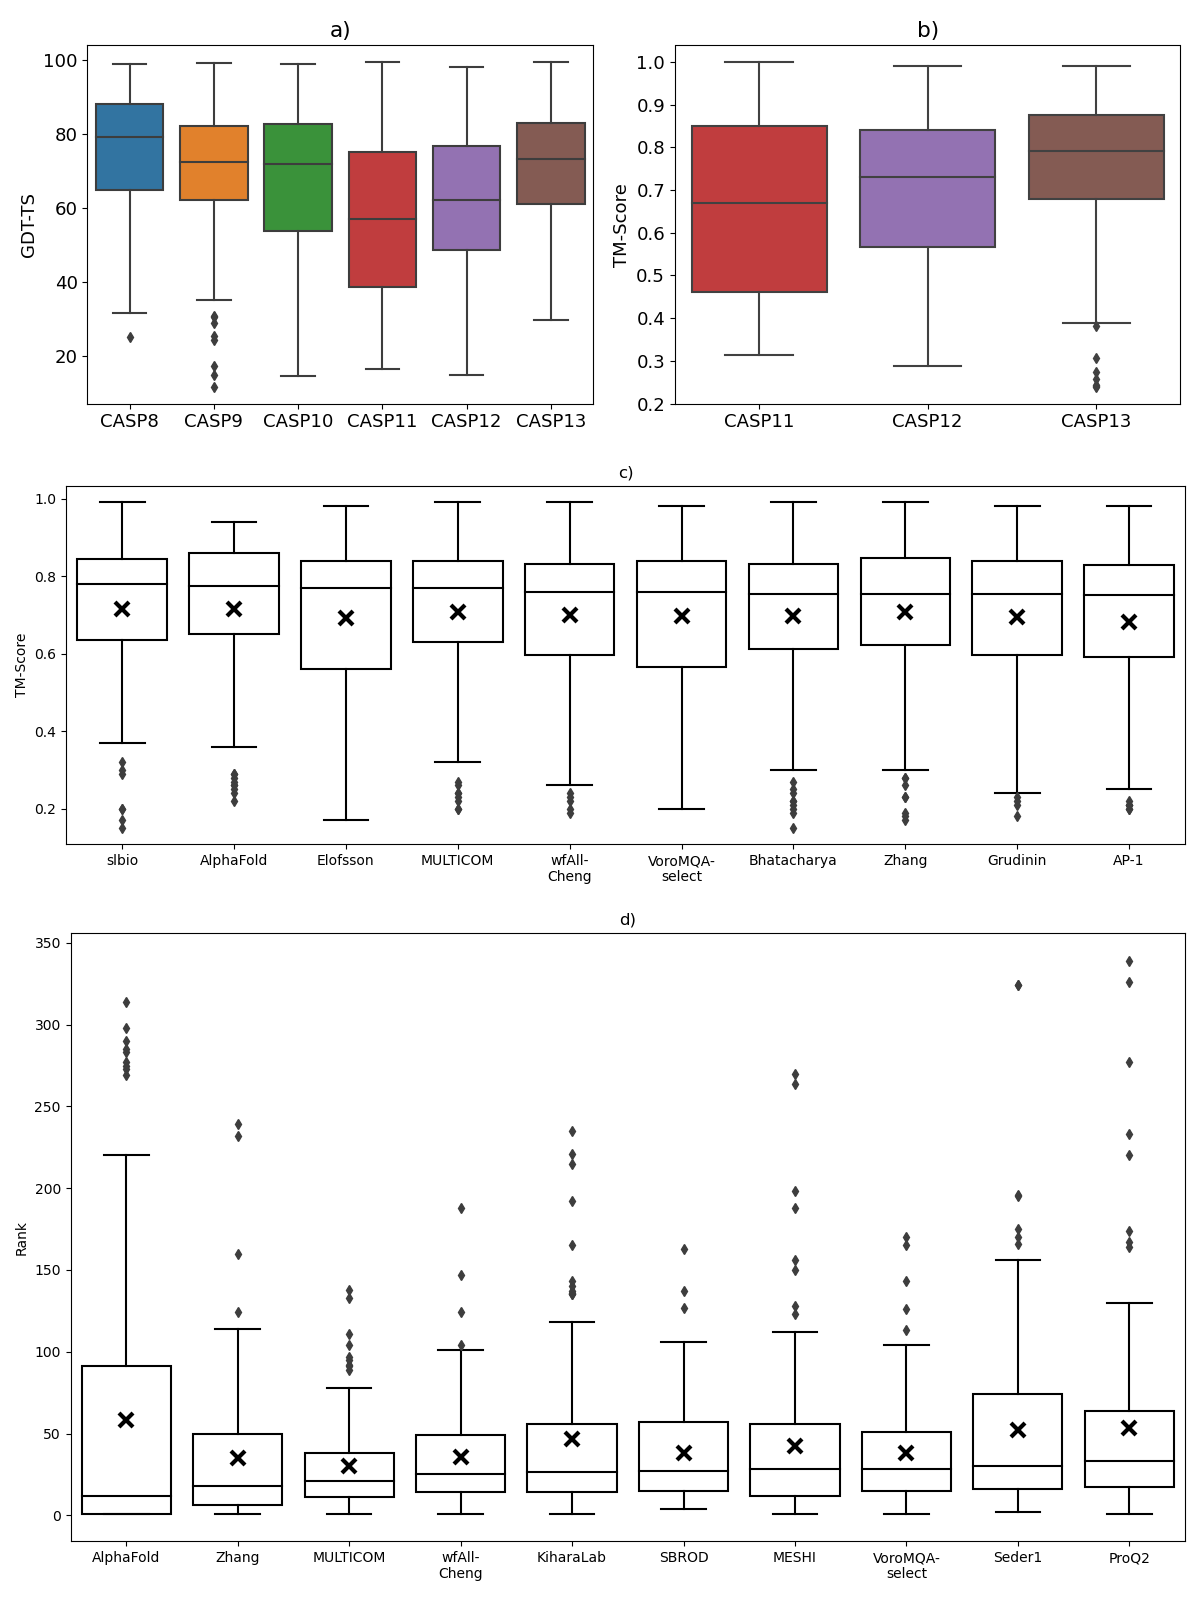
\includegraphics[scale=0.47]{imgs_tomas/casp_analysis_bw.png}
    \caption{Results from Previous CASP competitions in terms of GDT-TS (Global Distance Test - Total Score) - a), and TM-Score (Template Modelling) - b) of the regular targets (T). For each domain in each CASP competition, 10 best predictions were taken and their scores extracted. Only teams that submitted predictions for more than 19 domains were considered.
    Figure c) and d) summarize the results of best teams at CASP13 in terms of the TM-score - c) and TM-score based rank - d). For every domain, the TM-score was extracted and teams were ranked according to it. If a team uploaded more than 1 prediction, only the best one was taken. In both boxplots (c) and d)) the bar represents the median and the 'X' sign the mean. Data downloaded from: \cite{casp}}
    \label{fig:casp}
\end{figure}

CASP (Critical Assessment of protein Structure Prediction) is a biennial competition that reveals the progress in the field of computational structure prediction. 
Every two years competitors get access to a set of new protein sequences and are tasked to submit their predictions. 
The categories of the competition usually include:
\begin{itemize}
    \item Regular Targets (T)
    
    \begin{itemize}
        \item TBM - Template Based Modelling
        
        Targets for which at least one structural template can be found with a sequence search method such as PSI-Blast
        \item FM - Free Modelling
        
        Novel targets that can not rely on already known structures
        \item TBM/FM
        
        Targets that lie somewhere between the TBM and FM category
    \end{itemize}
    
    \item Refinement Targets (R)
    
        Measures the ability to refine targets after the first stage modelling phase. After the deadline for prediction of regular targets, the competitors will be given one of the best models for each protein with the task to further optimize/refine the structure.
        
    \item Other
    
    Assembly("how well current methods can determine domain-domain, subunit-subunit, and protein-protein interactions" \cite{casp}), Accuracy Estimation (assesses "the ability to provide useful accuracy estimates for the overall accuracy of models and at the domain and residue level" \cite{casp}), Contact prediction (introduced on CASP 13 - 2018), Distance prediction (on CASP 14 - 2020), Biological Relevance (CASP 14 - 2020) \cite{casp, casp13}
\end{itemize}

Figure \ref{fig:casp} a) and b) shows the results of protein predictions in terms of two scores: GDT-TS (Global Distance Test - Total Score) and TM-Score (Template Modelling Score) in the last 6 CASP competitions. 
For each competition, we extracted the best scores of best predictions for each domain, took their average and visualized the distribution with a boxplot.
Both scores are percentages (with GDT-TS multiplied by 100) and rely on structural alignment. 
The reason why simple mean squared distance is not favoured is because of its high sensitivity towards outliers. 
GDT-TS and TM-score account for this. 

For calculation of GDT-TS, many different local superpositions are taken to detect similarities between the two structures \cite{gdt1}. 
Scores below 30\% are considered random structures, scores above 50\% should have correct overall topology and structures with GDT-TS > 75\% are considered as good folds \cite{casp13}.

TM-score solves the outlier problem in a different way. 
First, it puts more weight on small distance errors than large distance errors and second, it takes into account the length of the sequence. 
Models with TM-scores lower than 0.17 are as good as random folds while models with TM-Score > 0.5 are considered as good folds \cite{tmscore}.

During CASP11 the prediction accuracy decreased, which is likely a result of ambiguous domain splits and difficult classification of domains into the TBM and FM categories. 
Many domains with low sequence similarity but high structural similarity contained deletions/insertions at the core, which subsequently decreased the prediction accuracy \cite{casp11}.

During CASP12 several teams adopted the idea (and showed its potential) of using contact maps to predict tertiary structure. 
This resulted in great improvement, especially for harder targets in the Free Modelling category. 
The contact precision increased from $\sim 27\%$ to $~47\%$ \cite{casp12}.

Teams participating in CASP13 pushed this accuracy to $70\%$, mainly due to the use of deep neural networks, with great dependence on the alignment depth. 
Another advance came through the prediction of inter-residue distance maps, which were then used as constraints to folding the protein. 
This idea was adopted by several teams, among which AlphaFold (A7D) predicted 42 domains out of 123, best out of all competitors. 
Even though this is an impressive result, looking at Figure \ref{fig:casp} c) and d) one can see that performance of other teams was similar to the performance of AlphaFold in terms of the TM-Score and the median rank. 
Deep learning pipelines of teams such as AlphaFold, RaptorX, were accompanied by teams implementing ideas such as fragment assembly (team Zhang \cite{zhang}), a combination of several features extracted from the structure from PDB database (Multicom \cite{multicom0}) or clever definition of statistical potential and good structure quality assessment (VoroMQA-select \cite{voromqa}).

The approach taken by AlphaFold relies heavily on the number of found homologs in sequence databases, which might be a reason for the large spread of median ranks in Figure \ref{fig:casp}.
